\documentclass[11pt, oneside]{article}   	% use "amsart" instead of "article" for AMSLaTeX format
\usepackage[margin=1in]{geometry}                		% See geometry.pdf to learn the layout options. There are lots.
\geometry{letterpaper}                   		% ... or a4paper or a5paper or ... 
\usepackage{graphicx}				% Use pdf, png, jpg, or eps§ with pdflatex; use eps in DVI mode
								% TeX will automatically convert eps --> pdf in pdflatex		
\usepackage{amssymb}
\usepackage{xcolor}
\usepackage{multirow}
\usepackage{fancyhdr}
\usepackage[normalem]{ulem}
%\usepackage{substack}
\usepackage{mathtools}
\usepackage{multirow}
\usepackage{url}
%SetFonts

\newcommand{\diru}{$\uparrow$}
\newcommand{\dirl}{$\leftarrow$}
\newcommand{\dird}{$\nwarrow$}
\newcommand{\dirdl}{$\substack{\nwarrow\\\leftarrow}$}
\newcommand{\dirdu}{$\substack{\uparrow\\\nwarrow}$}
\newcommand{\dirlu}{$\substack{\uparrow\\\leftarrow}$}
\newcommand{\dirdlu}{$\substack{\uparrow\\\nwarrow\\\leftarrow}$}

\newcommand{\dirui}{\rotatebox[origin=c]{90}{$\Rsh$}}
\newcommand{\dirdi}{\rotatebox[origin=c]{90}{$\Lsh$}}
\newcommand{\diruui}{\rotatebox[origin=c]{90}{$\Rsh$}}
\newcommand{\dirdui}{$\nwarrow$\rotatebox[origin=c]{90}{$\Rsh$}}
\newcommand{\dirlui}{$\leftarrow$\rotatebox[origin=c]{90}{$\Rsh$}}
\newcommand{\dirldi}{$\leftarrow$\rotatebox[origin=c]{90}{$\Lsh$}}
\newcommand{\dirddi}{$\nwarrow$\rotatebox[origin=c]{90}{$\Lsh$}}
\newcommand{\dirudi}{$\uparrow$\rotatebox[origin=c]{90}{$\Lsh$}}
\newcommand{\dirdiui}{\rotatebox[origin=c]{90}{$\Lsh\Rsh$}}
%SetFonts


\title{Midterm Exam}
\author{CS 4364/5364}
\date{Spring 2022}							% Activate to display a given date or no date
\pagestyle{fancy}
\lhead{CS 4364/5364 Midterm}
\rhead{Spring 2022}
%\rhead{Name:\hspace{15em}}

\begin{document}
\maketitle

\begin{center}
Name: \underline{ \hspace{20em} }
\end{center}
\paragraph{Instructions:}
Please read all of the instructions below before you begin:
\begin{itemize}
\item Read all of the questions in the exam before you begin. 
\item Questions marked with a dagger (\dag) are required for students in CS 5364, and bonus (optional) for those in CS 4364
\item Figures (pictograms) can be included if they help describe a solution, and are encouraged if they are clear. 
\item Remember that unanswered questions will receive 0 credit, any reasonable try at a response will receive at least half-credit. If you feel you're unable to provide a reasonable answer to a question, you can answer with ``I cannot provide a reasonable attempt for this question'', which will be provided quarter-credit. 
\item Students are allowed to bring any written material with them to the exam, but no electronic devices can be used during the exam. 
\item if you need extra room, please use the \emph{back of the previous page} rather than the current one (when it is folded open your whole answer should be showing). 
\end{itemize}

\begin{center}
\begin{tabular}{|c|c|c|c|}

\multicolumn{1}{c}{question/part} & \multicolumn{1}{c}{score} & \multicolumn{1}{c}{4364} & \multicolumn{1}{c}{5364}\\
\hline
1a & \hspace{5em} &/10 &/10\\ 
1b & \hspace{5em}&/5 &/5\\ 
1c & \hspace{5em}&/10 &/10\\ 
1d\dag & \hspace{5em}&     (bonus)&/10\\ 
\hline
2a & \hspace{5em}&/10 &/10\\ 
2b & \hspace{5em}&/5 &/5\\ 
2c & \hspace{5em}&/5 &/5\\ 
\hline
3a & \hspace{5em}&/12 &/12\\ 
3b\dag & \hspace{5em}&      (bonus)&/10\\ 
\hline
4a & \hspace{5em}&/6 &/6\\ 
4b & \hspace{5em}&/5 &/5\\ 
4c & \hspace{5em}&/4 &/4\\ 
\hline 
5\dag & \hspace{5em}&       (bonus)&/10\\ 
\hline
6 & \hspace{5em}&/15 &/15\\ 
\hline
\hline
\textbf{Total} & & /82 & /117\\
\hline
\end{tabular}
\end{center}

\clearpage
\begin{enumerate}
\item Use the \textit{Needleman-Wunch} dynamic programming table for $S = $ \texttt{TTTATG} and $T = $ \texttt{TCTAT} below to the next questions.
%
\renewcommand{\arraystretch}{2}
\begin{center}
{\footnotesize
\begin{tabular}{|c||c|c|c|c|c|c|c|c|c|}
\hline
& & \texttt{T} &  \texttt{T} &  \texttt{T} &  \texttt{A} &  \texttt{T} &  \texttt{G}\\
\hline
\hline
&  0 &	  \dirl -1 &	 \dirl  -2 &	\dirl -3 &	\dirl -4 &	\dirl -5 &	\dirl -6  \\[1ex]
\hline
\texttt{T} &  \diru -1 &	 \dird 8  &	 \dirdl 7 &	\dirdl 6 &	\dirl 5 &	\dirdl 4 &		\dirl 3  \\[1ex]
\hline 
\texttt{C} &  \diru -2 & 	\diru 7 & 	 \dirlu 6 &    \dirlu 5 & \dirlu 4 &		\dirlu 3 &	\dirlu 2 \\[1ex]
\hline
\texttt{T} &  \diru -3 & 	\dirdu 6 & \dird 15 & \dirdl 14 &  \dirl 13 & \dirdl 12 & \dirl 11 \\[1ex]
\hline 
\texttt{A} &  \diru -4 & \diru 5 & \diru 14 & \dirlu 13 &   \dird 22 & \dirl 21 & \dirl 20  \\[1ex]
\hline 
\texttt{T} &  \diru -5 & \dirdu 4 & \dirdu 13 & \dird 22 &   \dirlu 21 & \dird 30 & \dirl 29  \\[1ex]\hline 
\end{tabular}
}
\end{center}
\begin{enumerate}
\item (10 pts) How many co-optimal alignments of the two strings are there? What are they? 
\item (5 pts) What is the optimal alignment of $S[1....3]$ and $T[1...5]$? (note these are prefixes \texttt{TTT} and \texttt{TCTAT})
\item (10 pts) What is the indel penalty used to construct the table? match score?
\item \dag (10 pts/3 pts bonus) Can you determine the mismatch penalty from the table above? \textbf{Explain why or why not.}
\end{enumerate}

\clearpage 

\item Below is an algorithm description for a given problem (not defined on purpose). 

\begin{itemize}
\item assume you are given a string $S=s_1s_2s_3...s_n$.
\item set $S^R = s_ns_{n-1}s_{n-3}...s_1$, that is $S^R$ is the reverse of $S$.
\item construct a new string $T=S\$S^R$, where $\$\notin\Sigma$. 
\item compute the maximum prefix overlap, $M_i(T)$ for each $2 \le i \le (2n+1)$.
\item return $M_{n+2}(T) == n$.
\end{itemize}


\begin{enumerate}
\item (10 pts) What is returned when (i)$S=\texttt{ABCBA}$? (ii)$S=\texttt{ABCDBA}$?
\item (5 pts) What is the running time of the algorithm (in terms of $n$, the length of $S$)?
\item (5 pts) What does this algorithm do? 
\end{enumerate}

\clearpage

\item Given the alignments below, determine the number of matches, mismatches, gaps, and indels; place the counts in the table. (2 pt each)  

\begin{center}
\renewcommand{\arraystretch}{1}
\begin{tabular}{r|c|c|c|c|c|c|}
\multicolumn{1}{c}{} &\multicolumn{1}{c}{}  &  \multicolumn{1}{c}{} & \multicolumn{1}{c}{Matches} & \multicolumn{1}{c}{Mismatches} & \multicolumn{1}{c}{Gaps} & \multicolumn{1}{c}{Indels}\\
\multicolumn{1}{c}{} &\multicolumn{1}{c}{}  &  \multicolumn{1}{c}{} & \multicolumn{1}{c}{mt} & \multicolumn{1}{c}{ms} & \multicolumn{1}{c}{gp} & \multicolumn{1}{c}{id}\\
\cline{2-2} \cline{4-7} 
\multirow{2}{*}{$A_1$} & \texttt{GCT-AC-TTGC} & \hspace{2em} & \hspace{5em} & \hspace{5em} & \hspace{5em} & \hspace{5em} \\
& \texttt{-CTG-CA-TGC}  & & & & & \\
\cline{2-2} \cline{4-7} 
\multirow{2}{*}{$A_2$} & \texttt{GCTACTTGC} & & & & &\\
& \texttt{-CTGCATGC}  & & & & &\\
\cline{2-2} \cline{4-7} 
\multirow{2}{*}{$A_3$} & \texttt{GCT--ACTTGC}  & & & & &\\
& \texttt{-CTGCA--TGC} & & & & &\\
\cline{2-2} \cline{4-7} 
\end{tabular}
\end{center}

\dag (10 pts/3 pts bonus) Determine at set of values for $\alpha, \beta, \gamma$, and $\delta$ such that each of the alignments $A_3$ is optimal under the following scoring:
\[
\alpha\text{mt} + \beta\text{ms} + \gamma\text{gp} + \delta\text{id}
\]
assuming $A_1,A_2,$ and $A_3$ are the only possible alignments of the two sequences. 

\begin{center}
\begin{tabular}{|c|c|c|c|}
\multicolumn{1}{c}{$\alpha$} & \multicolumn{1}{c}{$\beta$} & \multicolumn{1}{c}{$\gamma$} & \multicolumn{1}{c}{$\delta$}\\
\hline
\hspace{5em} & \hspace{5em} & \hspace{5em} & \hspace{5em} \\
\hspace{5em} & \hspace{5em} & \hspace{5em} & \hspace{5em} \\
\hline
\end{tabular}
\end{center}

\clearpage
\item Use the generalized suffix tree below to answer the next questions. 
\label{q:SuffTree}

\begin{figure}[h!]
\centering
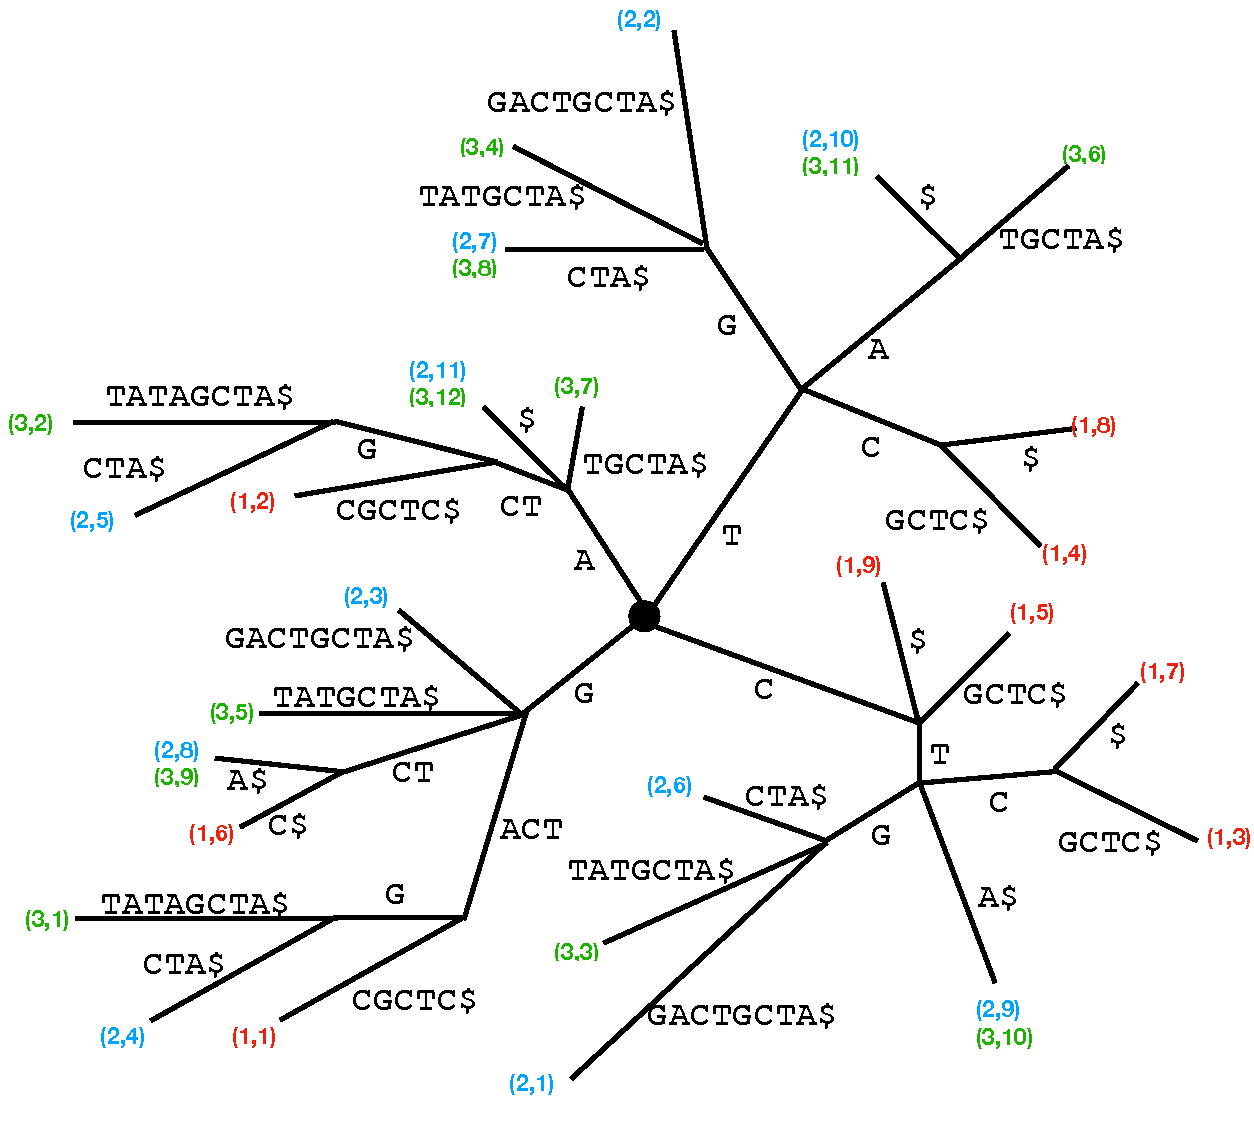
\includegraphics[width=0.75\textwidth]{GST}
\label{f:SuffTree}
\caption{Suffix tree for question~\ref{q:SuffTree}}
\end{figure}

\begin{enumerate}
\item (6 pts) What are the 3 strings encoded in the tree?
\item (5 pts) What is the longest string contained in  \textbf{at least two} strings? 
\item (4 pts) Name two possible alphabets that could be used to produce the strings used to construct the strings? 
\end{enumerate}

\clearpage
\item \dag (10 pts/3 pts bonus) True or False: For global pairwise alignment of two strings of size $m$ and $n$
\[2\text{mt} + 2\text{ms} + \text{id} + \text{gp} = (m+n).\] 
Where mt is the count of matches, ms is the count of mismatches, and id is the number of indels, and gp is the number of gaps.
\textbf{Explain your answer.}  

\clearpage
\item (15 pts)
Given two sequences $S$ and $T$ (not necessarily the same length), 
let $G$ and $L$ be the scores of an optimal global alignment and an optimal local alignment, respectively.
\begin{enumerate}
\item True or false ---  $\forall S,T\in\Sigma^*: L \ge G$. \textbf{Explain your answer.}  

\end{enumerate}

\end{enumerate}

\end{document} 